\documentclass[12pt,a4paper]{article}

% ─── Page Layout ───────────────────────────────────────────────────────────────
\usepackage[a4paper, margin=0.8in, headheight=14pt]{geometry}

% ─── Fonts (XeLaTeX) ───────────────────────────────────────────────────────────
\usepackage{fontspec}
\usepackage{unicode-math}
\setmainfont{TeX Gyre Pagella}
\setmonofont[Scale=0.88]{TeX Gyre Cursor}
\setmathfont{Latin Modern Math}

% ─── Packages ──────────────────────────────────────────────────────────────────
\usepackage{xcolor}
\usepackage{colortbl}
\usepackage{titlesec}
\usepackage{enumitem}
\usepackage{tabularx}
\usepackage{booktabs}
\usepackage{array}
\usepackage{amsmath}
\usepackage{tikz}
\usetikzlibrary{shapes.geometric, arrows.meta, positioning, calc, fit}
\usepackage{tcolorbox}
\tcbuselibrary{skins, breakable}
\usepackage{hyperref}
\usepackage{fancyhdr}
\usepackage{graphicx}
\usepackage{microtype}
\usepackage{caption}
\usepackage{setspace}
\usepackage{multirow}
\usepackage{tocloft}

% ─── Q&A helper ────────────────────────────────────────────────────────────────
\newcommand{\Q}[1]{\textbf{#1}\par\noindent\ignorespaces}

% ─── Colour Palette ────────────────────────────────────────────────────────────
\definecolor{myred}{RGB}{196,30,58}
\definecolor{mydark}{RGB}{30,30,50}
\definecolor{mygreen}{RGB}{14,120,80}
\definecolor{myteal}{RGB}{0,130,140}
\definecolor{myamber}{RGB}{180,100,0}
\definecolor{mypurple}{RGB}{100,30,160}
\definecolor{mygray}{RGB}{246,247,249}
\definecolor{mgframe}{RGB}{180,185,200}
\definecolor{watermark}{RGB}{195,200,215}
\definecolor{hdrred}{RGB}{250,232,235}
\definecolor{hdrgreen}{RGB}{220,244,233}
\definecolor{hdrteal}{RGB}{220,242,244}
\definecolor{hdramber}{RGB}{253,242,215}
\definecolor{hdrpurple}{RGB}{238,228,255}
\definecolor{hdrgray}{RGB}{238,240,245}
\definecolor{rowalt}{RGB}{250,251,253}

% ─── Section Formatting ────────────────────────────────────────────────────────
\titleformat{\section}
  {\large\bfseries\color{myred}}{\thesection.}{0.5em}{}
  [\vspace{1pt}{\color{myred}\rule{\linewidth}{0.8pt}}]
\titleformat{\subsection}
  {\normalsize\bfseries\color{mydark}}{\thesubsection}{0.5em}{}
\titlespacing*{\section}{0pt}{18pt}{7pt}
\titlespacing*{\subsection}{0pt}{11pt}{4pt}

\setlength{\parindent}{0pt}
\setlength{\parskip}{4pt}

% ─── TOC Styling ───────────────────────────────────────────────────────────────
\renewcommand{\cfttoctitlefont}{\large\bfseries\color{myred}}
\renewcommand{\cftaftertoctitle}{\par\noindent{\color{myred}\rule{\linewidth}{0.8pt}}}
\setlength{\cftbeforetoctitleskip}{0pt}
\setlength{\cftaftertoctitleskip}{6pt}
\renewcommand{\cftsecfont}{\normalsize\bfseries\color{mydark}}
\renewcommand{\cftsecpagefont}{\normalsize\bfseries\color{myteal}}
\renewcommand{\cftsecleader}{\cftdotfill{\cftdotsep}}
\setlength{\cftbeforesecskip}{7pt}
\renewcommand{\cftsubsecfont}{\small\color{mydark}}
\renewcommand{\cftsubsecpagefont}{\small\color{myteal}}
\setlength{\cftbeforesubsecskip}{3pt}
\setlength{\cftsubsecindent}{1.4em}

% ─── Table helpers ─────────────────────────────────────────────────────────────
\renewcommand{\arraystretch}{1.45}
\setlength{\tabcolsep}{6pt}
\newcolumntype{B}[1]{>{\small\bfseries\raggedright\arraybackslash}p{#1}}

% ─── Header / Footer ───────────────────────────────────────────────────────────
\pagestyle{fancy}
\fancyhf{}
\fancyhead[L]{\small\color{myred}\textbf{EC601}\;\color{mydark}--- Control System}
\fancyhead[R]{\small\color{myteal}\textbf{Module 4 Notes}}
\fancyfoot[C]{\small\color{mydark}\thepage}
\fancyfoot[R]{\small\color{watermark}\textit{© Biraj}}
\renewcommand{\headrulewidth}{0.5pt}
\renewcommand{\footrulewidth}{0.3pt}

% ─── Hyperref ──────────────────────────────────────────────────────────────────
\hypersetup{
  colorlinks=true, linkcolor=myteal, urlcolor=myteal,
  pdfauthor={Biraj Sarkar},
  pdftitle={EC601 --- Module 4 Notes}
}

% ─── tcolorbox styles ──────────────────────────────────────────────────────────
\tcbset{
  tikzbox/.style={
    colback=mygray, colframe=mgframe, boxrule=0.6pt, arc=4pt,
    left=8pt, right=8pt, top=6pt, bottom=6pt,
    colbacktitle=mgframe, coltitle=mydark, fonttitle=\small\bfseries
  },
  defbox/.style={
    colback=hdrgreen, colframe=mygreen, boxrule=0.8pt, arc=4pt,
    left=9pt, right=9pt, top=6pt, bottom=6pt,
    colbacktitle=mygreen, coltitle=white, fonttitle=\small\bfseries
  },
  formulabox/.style={
    colback=hdrteal, colframe=myteal, boxrule=0.8pt, arc=4pt,
    left=9pt, right=9pt, top=7pt, bottom=7pt,
    colbacktitle=myteal, coltitle=white, fonttitle=\small\bfseries
  },
  examplebox/.style={
    colback=hdramber, colframe=myamber, boxrule=0.8pt, arc=4pt,
    left=9pt, right=9pt, top=6pt, bottom=6pt,
    colbacktitle=myamber, coltitle=white, fonttitle=\small\bfseries
  },
  masonbox/.style={
    colback=hdrpurple, colframe=mypurple, boxrule=0.8pt, arc=4pt,
    left=9pt, right=9pt, top=6pt, bottom=6pt,
    colbacktitle=mypurple, coltitle=white, fonttitle=\small\bfseries
  },
  exambox/.style={
    colback=hdrpurple, colframe=mypurple, boxrule=1pt, arc=5pt,
    left=10pt, right=10pt, top=8pt, bottom=8pt,
    colbacktitle=mypurple, coltitle=white, fonttitle=\bfseries,
    breakable
  }
}
% Allow all boxes to break across pages — prevents footer overflow
\tcbset{breakable}

% ─── TikZ styles ───────────────────────────────────────────────────────────────
\tikzset{
  block/.style={rectangle, draw=myteal, fill=hdrteal,
    text width=2.6cm, align=center, minimum height=0.9cm,
    font=\small, rounded corners=3pt, line width=0.7pt},
  arrow/.style={-Stealth, thick, color=mydark},
  redarrow/.style={-Stealth, thick, color=myred},
  greenarrow/.style={-Stealth, thick, color=mygreen},
  line/.style={thick, color=mydark},
  axis/.style={-Stealth, thin, color=mydark},
  gridline/.style={thin, color=mgframe, dashed}
}

% ═══════════════════════════════════════════════════════════════════════════════
\begin{document}
% ═══════════════════════════════════════════════════════════════════════════════

\begin{center}
  {\LARGE\bfseries\color{myred} EC601 --- Control System}\\[5pt]
  {\normalsize\color{mydark} Semester VI \quad$\bullet$\quad 3L:0T:0P \quad$\bullet$\quad 3 Credits}\\[3pt]
  {\normalsize\color{myteal}\textbf{Module 4 Exam Notes}}\\[3pt]
  {\small\color{mydark} CGEC \;$|$\; B.Tech ECE (2023--27) \;$|$\; \textit{Biraj Sarkar}}
\end{center}
\vspace{2pt}
\noindent{\color{myred}\rule{\linewidth}{1.5pt}}
\vspace{2pt}

\tableofcontents
\newpage

%═══════════════════════════════════════════════════════════════════════════════
\section{Frequency Response Analysis --- Introduction}
%═══════════════════════════════════════════════════════════════════════════════

\textbf{Frequency response analysis} studies how a system responds to sinusoidal inputs of varying frequency. For a stable LTI system with transfer function $G(j\omega)$, a sinusoidal input $r(t)=A\sin(\omega t)$ produces a steady-state output $c(t)=A|G(j\omega)|\sin(\omega t + \angle G(j\omega))$.

\begin{tcolorbox}[defbox]
\textbf{Frequency Response Function:} Obtained by substituting $s = j\omega$ in the transfer function:
$$G(j\omega) = G(s)\big|_{s=j\omega} = |G(j\omega)|\,\angle\phi(\omega)$$
\textbf{Magnitude:} $|G(j\omega)|$ --- ratio of output to input amplitude.\\
\textbf{Phase:} $\phi(\omega) = \angle G(j\omega)$ --- phase shift of output relative to input.
\end{tcolorbox}

\begin{tabularx}{\linewidth}{|B{3.2cm}|X|}
\hline
\rowcolor{hdrteal}
\multicolumn{1}{|>{\centering\arraybackslash}p{3.2cm}|}{\textbf{\color{myteal}Plot Type}} &
\multicolumn{1}{>{\centering\arraybackslash}X|}{\textbf{\color{myteal}Description}} \\
\hline
Polar Plot & Locus of $G(j\omega)$ in the complex plane as $\omega: 0\to\infty$. Also called Nyquist plot (open-loop). \\
\hline
\rowcolor{rowalt}
Bode Plot & Two separate plots: $|G(j\omega)|$ in dB vs $\log\omega$, and $\angle G(j\omega)$ in degrees vs $\log\omega$. \\
\hline
Nyquist Plot & Polar plot of $G(j\omega)H(j\omega)$ for $\omega: -\infty\to+\infty$; used for Nyquist stability criterion. \\
\hline
\rowcolor{rowalt}
Nichols Chart & Magnitude vs phase plot; used for closed-loop frequency response from open-loop data. \\
\hline
\end{tabularx}

%═══════════════════════════════════════════════════════════════════════════════
\section{Polar Plots}
%═══════════════════════════════════════════════════════════════════════════════

\begin{tcolorbox}[defbox]
\textbf{Polar Plot:} A plot of $G(j\omega)$ in the complex ($\text{Re}$--$\text{Im}$) plane as $\omega$ varies from $0$ to $+\infty$. Each point on the curve represents the tip of the phasor $G(j\omega)$ at a particular frequency. The distance from the origin is $|G(j\omega)|$ and the angle is $\angle G(j\omega)$.
\end{tcolorbox}

\subsection{Polar Plot of Standard Factors}

\begin{tabularx}{\linewidth}{|B{3.4cm}|>{\centering\arraybackslash}X|>{\centering\arraybackslash}X|}
\hline
\rowcolor{hdrteal}
\multicolumn{1}{|>{\centering\arraybackslash}p{3.4cm}|}{\textbf{\color{myteal}Factor}} &
\textbf{\color{myteal}At $\omega=0$} & \textbf{\color{myteal}At $\omega\to\infty$} \\
\hline
$K$ (gain) & $(K, 0°)$ & $(K, 0°)$ --- point on real axis \\
\hline
\rowcolor{rowalt}
$j\omega$ (integrator) & $\infty\angle{-90°}$ & $0\angle{-90°}$ --- negative imaginary axis \\
\hline
$1/j\omega$ & $\infty\angle{-90°}$ & $0\angle{-90°}$ --- negative imaginary axis \\
\hline
\rowcolor{rowalt}
$1/(1+j\omega T)$ & $(1, 0°)$ & $(0, -90°)$ --- 4th quadrant semicircle \\
\hline
$1/(j\omega)^2$ & $\infty\angle{-180°}$ & $0\angle{-180°}$ --- negative real axis \\
\hline
\rowcolor{rowalt}
$1/[j\omega(1+j\omega T)]$ & $\infty\angle{-90°}$ & $0\angle{-180°}$ --- 3rd quadrant \\
\hline
\end{tabularx}

\subsection{Key Properties of Polar Plots}

\begin{itemize}[leftmargin=*, itemsep=3pt]
  \item The \textbf{starting point} ($\omega=0$) and \textbf{ending point} ($\omega\to\infty$) are determined by the system type and order.
  \item For a \textbf{Type 0} system: starts on positive real axis; for \textbf{Type 1}: starts at $-90°$ infinity; for \textbf{Type 2}: starts at $-180°$ infinity.
  \item The \textbf{number of clockwise encirclements} of the $(-1, j0)$ point determines closed-loop stability (Nyquist criterion).
  \item The \textbf{gain crossover frequency} $\omega_{gc}$: where $|G(j\omega)|=1$ (0 dB).
  \item The \textbf{phase crossover frequency} $\omega_{pc}$: where $\angle G(j\omega) = -180°$.
\end{itemize}

\begin{tcolorbox}[tikzbox, title={Polar Plot --- Type 1, Second Order: $G(j\omega)=K/[j\omega(1+j\omega T)]$}]
\centering
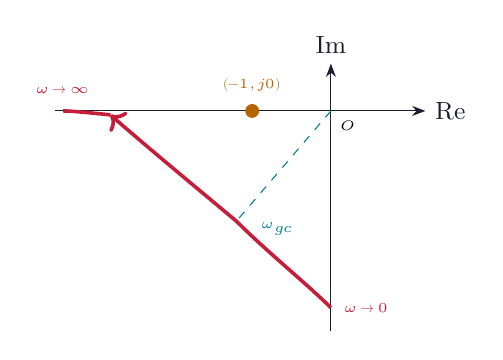
\begin{tikzpicture}[scale=1.0]
  % Axes
  \draw[axis] (-3.5,0) -- (1.2,0) node[right,font=\small] {Re};
  \draw[axis] (0,-2.8) -- (0,0.6) node[above,font=\small] {Im};
  % Curve: starts at -90 deg infinity, sweeps to origin at -180 deg
  \draw[color=myred, line width=1.3pt, ->]
    (0,-2.5) .. controls (-0.3,-2.2) and (-0.8,-1.8) .. (-1.2,-1.4)
    .. controls (-1.8,-0.9) and (-2.4,-0.4) .. (-2.8,-0.05);
  \draw[color=myred, line width=1.3pt]
    (-2.8,-0.05) .. controls (-3.1,-0.02) and (-3.3,0) .. (-3.4,0);
  % Labels
  \node[right, font=\tiny, color=myred] at (0.05,-2.5) {$\omega\to 0$};
  \node[above, font=\tiny, color=myred] at (-3.4,0.1) {$\omega\to\infty$};
  % -1,0 point
  \fill[myamber] (-1,0) circle (2.5pt);
  \node[above, font=\tiny, color=myamber] at (-1,0.12) {$(-1,j0)$};
  % Gain crossover
  \draw[dashed, color=myteal, thin] (0,0) -- (-1.2,-1.4);
  \node[right, font=\tiny, color=myteal] at (-1.0,-1.5) {$\omega_{gc}$};
  % Origin
  \node[below right, font=\tiny] at (0,0) {$O$};
\end{tikzpicture}
\end{tcolorbox}

%═══════════════════════════════════════════════════════════════════════════════
\section{Bode Plot}
%═══════════════════════════════════════════════════════════════════════════════

\begin{tcolorbox}[defbox]
\textbf{Bode Plot:} Two semi-log plots of the open-loop frequency response $G(j\omega)$:
\begin{itemize}[leftmargin=*, itemsep=2pt, topsep=2pt]
  \item \textbf{Magnitude plot:} $20\log_{10}|G(j\omega)|$ in \textbf{dB} vs $\log_{10}\omega$ (log scale).
  \item \textbf{Phase plot:} $\angle G(j\omega)$ in \textbf{degrees} vs $\log_{10}\omega$ (log scale).
\end{itemize}
Bode plots use \textbf{asymptotic approximations} (straight-line segments) for quick sketching.
\end{tcolorbox}

\subsection{Standard Factors and Their Bode Contributions}

\begin{tabularx}{\linewidth}{|B{3.0cm}|>{\centering\arraybackslash}X|>{\centering\arraybackslash}X|}
\hline
\rowcolor{hdrteal}
\multicolumn{1}{|>{\centering\arraybackslash}p{3.0cm}|}{\textbf{\color{myteal}Factor}} &
\textbf{\color{myteal}Magnitude (dB)} & \textbf{\color{myteal}Phase} \\
\hline
Gain $K$ & $20\log K$ (constant) & $0°$ (if $K>0$); $-180°$ (if $K<0$) \\
\hline
\rowcolor{rowalt}
$j\omega$ (zero at origin) & $+20$ dB/dec, passes through 0 dB at $\omega=1$ & $+90°$ (constant) \\
\hline
$1/j\omega$ (pole at origin) & $-20$ dB/dec, passes through 0 dB at $\omega=1$ & $-90°$ (constant) \\
\hline
\rowcolor{rowalt}
$(1+j\omega T)$ (simple zero) & $0$ dB for $\omega\ll1/T$; $+20$ dB/dec for $\omega\gg1/T$ & $0°\to+90°$, $45°$ at $\omega=1/T$ \\
\hline
$1/(1+j\omega T)$ (simple pole) & $0$ dB for $\omega\ll1/T$; $-20$ dB/dec for $\omega\gg1/T$ & $0°\to-90°$, $-45°$ at $\omega=1/T$ \\
\hline
\rowcolor{rowalt}
$1/(j\omega)^2$ (double pole) & $-40$ dB/dec & $-180°$ (constant) \\
\hline
2nd order factor & $0$ dB below $\omega_n$; $-40$ dB/dec above $\omega_n$; resonance peak near $\omega_n$ & $0°\to-180°$, $-90°$ at $\omega_n$ \\
\hline
\end{tabularx}

\subsection{Corner Frequency (Break Frequency)}

\begin{tcolorbox}[formulabox, title={Corner Frequency}]
For a factor $(1+j\omega T)$: \textbf{corner frequency} $\omega_c = 1/T$ rad/s.\\[4pt]
\textbf{Asymptotic error at corner frequency:}
\begin{itemize}[leftmargin=*, itemsep=2pt, topsep=2pt]
  \item Magnitude: actual value differs from asymptote by $\pm 3$ dB at $\omega = \omega_c$.
  \item Phase: actual $= \pm 45°$ at $\omega_c$; asymptote approximation has $\pm 5.7°$ max error.
\end{itemize}
\end{tcolorbox}

\subsection{Bode Plot Sketching Procedure}

\begin{enumerate}[label=\textbf{Step \arabic*:}, leftmargin=2.5cm, itemsep=3pt]
  \item Write $G(j\omega)$ in \textbf{time-constant form}: factor out constants, express each factor as $(1+j\omega T)$.
  \item Compute the \textbf{initial slope}: $-20N$ dB/dec where $N$ = system type (number of poles at origin).
  \item Mark all \textbf{corner frequencies} $\omega_c = 1/T$ on the $\omega$-axis.
  \item Draw the \textbf{magnitude asymptotes}: slope changes by $+20$ dB/dec at each zero corner, $-20$ dB/dec at each pole corner.
  \item Apply \textbf{3 dB corrections} at each corner frequency if accuracy is needed.
  \item Draw the \textbf{phase plot}: sum contributions from each factor; use $\pm45°$/decade approximation.
\end{enumerate}

\begin{tcolorbox}[examplebox, title={Example: $G(j\omega) = \dfrac{10}{j\omega(1+0.1j\omega)(1+0.5j\omega)}$}]
\textbf{Factors:} Gain $K=10$ ($+20$ dB), pole at origin ($-20$ dB/dec from start), poles at $\omega_c=10$ and $\omega_c=2$.

\textbf{Initial value:} At $\omega=1$: $20\log(10/1) = 20$ dB (from gain and pole at origin).

\textbf{Slope changes:}
\begin{itemize}[leftmargin=*, itemsep=1pt, topsep=0pt]
  \item $\omega < 2$: slope $= -20$ dB/dec (one pole at origin)
  \item $2 < \omega < 10$: slope $= -40$ dB/dec (pole at $\omega=2$ adds $-20$)
  \item $\omega > 10$: slope $= -60$ dB/dec (pole at $\omega=10$ adds another $-20$)
\end{itemize}

\textbf{Phase:} $-90°$ (pole at origin) $-\tan^{-1}(0.5\omega) - \tan^{-1}(0.1\omega)$
\end{tcolorbox}

\begin{tcolorbox}[tikzbox, title={Bode Magnitude Plot Sketch}]
\centering
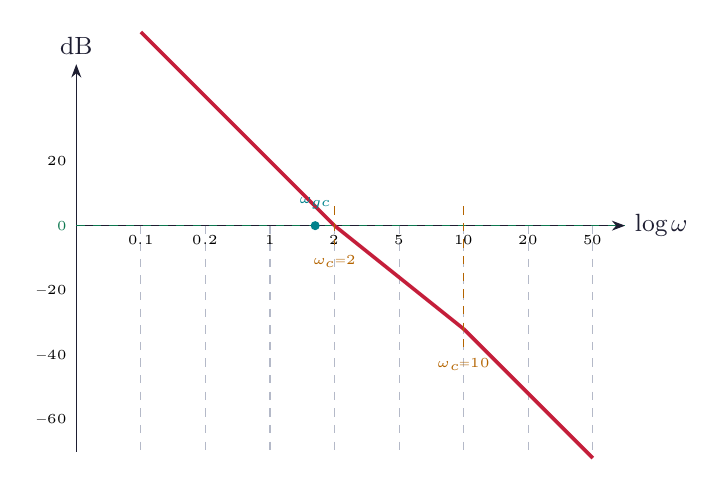
\begin{tikzpicture}[scale=0.82]
  % Axes
  \draw[axis] (0,0) -- (8.5,0) node[right,font=\small] {$\log\omega$};
  \draw[axis] (0,-3.5) -- (0,2.5) node[above,font=\small] {dB};
  % Grid lines
  \foreach \x in {1,2,3,4,5,6,7,8} \draw[gridline] (\x,0) -- (\x,-3.5);
  % Frequency labels
  \node[below,font=\tiny] at (1,0) {$0.1$};
  \node[below,font=\tiny] at (2,0) {$0.2$};
  \node[below,font=\tiny] at (3,0) {$1$};
  \node[below,font=\tiny] at (4,0) {$2$};
  \node[below,font=\tiny] at (5,0) {$5$};
  \node[below,font=\tiny] at (6,0) {$10$};
  \node[below,font=\tiny] at (7,0) {$20$};
  \node[below,font=\tiny] at (8,0) {$50$};
  % 0 dB line
  \draw[dashed, color=mygreen, thin] (0,0) -- (8.5,0);
  \node[left,font=\tiny,color=mygreen] at (0,0) {$0$};
  \node[left,font=\tiny] at (0,1) {$20$};
  \node[left,font=\tiny] at (0,-1) {$-20$};
  \node[left,font=\tiny] at (0,-2) {$-40$};
  \node[left,font=\tiny] at (0,-3) {$-60$};
  % Asymptote: -20dB/dec from start, passes through 20dB at w=1 (x=3)
  % At x=1 (w=0.1): 20+20*2=60dB -> y=3; at x=3 (w=1): 20dB -> y=1
  \draw[color=myred, line width=1.3pt] (1,3) -- (4,0);   % -20dB/dec until w=2
  % Corner at w=2 (x=4): slope becomes -40dB/dec
  \draw[color=myred, line width=1.3pt] (4,0) -- (6,-1.6); % -40dB/dec until w=10
  % Corner at w=10 (x=6): slope becomes -60dB/dec
  \draw[color=myred, line width=1.3pt] (6,-1.6) -- (8,-3.6); % -60dB/dec
  % Corner markers
  \draw[dashed,color=myamber,thin] (4,0.3) -- (4,-0.3) node[below,font=\tiny,color=myamber] {$\omega_c{=}2$};
  \draw[dashed,color=myamber,thin] (6,0.3) -- (6,-1.9) node[below,font=\tiny,color=myamber] {$\omega_c{=}10$};
  % Gain crossover
  \fill[myteal] (3.7,0) circle (2pt);
  \node[above,font=\tiny,color=myteal] at (3.7,0.1) {$\omega_{gc}$};
\end{tikzpicture}
\end{tcolorbox}

%═══════════════════════════════════════════════════════════════════════════════
\section{Stability in Frequency Domain}
%═══════════════════════════════════════════════════════════════════════════════

\subsection{Gain Margin (GM)}

\begin{tcolorbox}[defbox]
\textbf{Gain Margin:} The factor by which the open-loop gain can be \textit{increased} before the closed-loop system becomes unstable. Measured at the \textbf{phase crossover frequency} $\omega_{pc}$ (where $\angle G(j\omega)H(j\omega) = -180°$).
$$GM = \frac{1}{|G(j\omega_{pc})H(j\omega_{pc})|}$$
In dB: $GM_{dB} = -20\log_{10}|G(j\omega_{pc})H(j\omega_{pc})|$\\[4pt]
\textbf{Stable system:} $GM > 1$ (i.e., $GM_{dB} > 0$ dB). \quad \textbf{Unstable:} $GM < 1$ ($GM_{dB} < 0$ dB).
\end{tcolorbox}

\subsection{Phase Margin (PM)}

\begin{tcolorbox}[defbox]
\textbf{Phase Margin:} The additional phase lag that can be introduced before the closed-loop system becomes unstable. Measured at the \textbf{gain crossover frequency} $\omega_{gc}$ (where $|G(j\omega)H(j\omega)| = 1$, i.e., 0 dB).
$$PM = 180° + \angle G(j\omega_{gc})H(j\omega_{gc})$$
\textbf{Stable system:} $PM > 0°$. \quad \textbf{Unstable:} $PM < 0°$.\\[4pt]
\textbf{Typical design target:} $GM \geq 6$ dB, $PM \geq 30°$--$60°$.
\end{tcolorbox}

\begin{tcolorbox}[tikzbox, title={GM and PM on Bode Plot}]
\centering
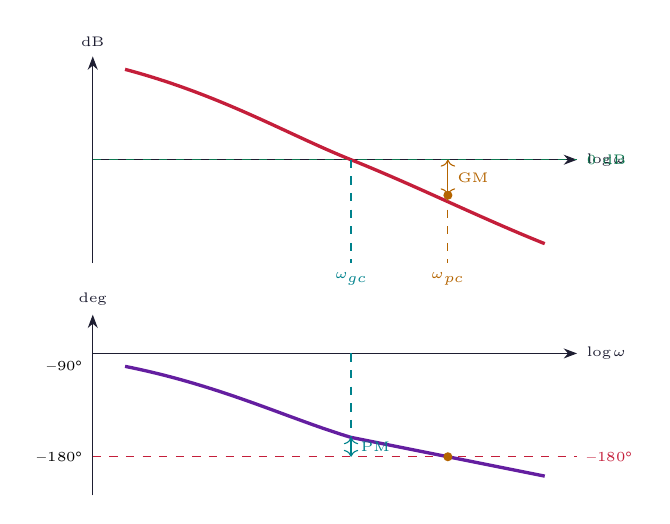
\begin{tikzpicture}[scale=0.82]
  % ── Magnitude plot ──
  \draw[axis] (0,1.8) -- (7.5,1.8) node[right,font=\tiny] {$\log\omega$};
  \draw[axis] (0,0.2) -- (0,3.4) node[above,font=\tiny] {dB};
  \draw[dashed,color=mygreen,thin] (0,1.8) -- (7.5,1.8) node[right,font=\tiny,color=mygreen] {0 dB};
  % Magnitude curve
  \draw[color=myred,line width=1.2pt]
    (0.5,3.2) .. controls (2,2.8) and (3,2.2) .. (4,1.8)
    .. controls (5,1.4) and (6,0.9) .. (7,0.5);
  % wgc marker
  \draw[dashed,color=myteal,thin] (4,1.8) -- (4,0.2) node[below,font=\tiny,color=myteal] {$\omega_{gc}$};
  % wpc marker
  \draw[dashed,color=myamber,thin] (5.5,1.8) -- (5.5,0.2) node[below,font=\tiny,color=myamber] {$\omega_{pc}$};
  % GM arrow
  \draw[<->,color=myamber,thin] (5.5,1.8) -- (5.5,1.25);
  \node[right,font=\tiny,color=myamber] at (5.5,1.52) {GM};
  \fill[myamber] (5.5,1.25) circle (2pt);
  % ── Phase plot ──
  \draw[axis] (0,-1.2) -- (7.5,-1.2) node[right,font=\tiny] {$\log\omega$};
  \draw[axis] (0,-3.4) -- (0,-0.6) node[above,font=\tiny] {deg};
  \draw[dashed,color=myred,thin] (0,-2.8) -- (7.5,-2.8) node[right,font=\tiny,color=myred] {$-180°$};
  % Phase curve
  \draw[color=mypurple,line width=1.2pt]
    (0.5,-1.4) .. controls (2,-1.7) and (3,-2.2) .. (4,-2.5)
    .. controls (5,-2.7) and (5.5,-2.8) .. (7,-3.1);
  % PM arrow at wgc
  \draw[<->,color=myteal,thin] (4,-2.5) -- (4,-2.8);
  \node[right,font=\tiny,color=myteal] at (4,-2.65) {PM};
  \draw[dashed,color=myteal,thin] (4,-1.2) -- (4,-2.5);
  % -180 at wpc
  \fill[myamber] (5.5,-2.8) circle (2pt);
  \node[left,font=\tiny] at (0,-1.4) {$-90°$};
  \node[left,font=\tiny] at (0,-2.8) {$-180°$};
\end{tikzpicture}
\end{tcolorbox}

\begin{tabularx}{\linewidth}{|B{3.2cm}|>{\centering\arraybackslash}X|>{\centering\arraybackslash}X|}
\hline
\rowcolor{hdrgray}
\multicolumn{1}{|>{\centering\arraybackslash}p{3.2cm}|}{\textbf{Margin}} &
\textbf{\color{myamber}Definition} & \textbf{\color{mygreen}Measurement Point} \\
\hline
Gain Margin (GM) & $1/|G(j\omega_{pc})|$ & At phase crossover freq $\omega_{pc}$ ($\angle = -180°$) \\
\hline
\rowcolor{rowalt}
Phase Margin (PM) & $180° + \angle G(j\omega_{gc})$ & At gain crossover freq $\omega_{gc}$ ($|G|=1$) \\
\hline
Stable condition & $GM > 1$ ($>0$ dB) & $PM > 0°$ \\
\hline
\rowcolor{rowalt}
Good design & $GM \geq 6$ dB & $PM = 30°$--$60°$ \\
\hline
\end{tabularx}

\begin{tcolorbox}[exambox, title={Exam Tips --- GM and PM}]
\begin{itemize}[leftmargin=*, itemsep=3pt, topsep=0pt]
  \item \textbf{GM} is read from the magnitude plot at $\omega_{pc}$; \textbf{PM} is read from the phase plot at $\omega_{gc}$.
  \item If the magnitude curve \textit{never} crosses 0 dB, $\omega_{gc}$ does not exist --- system is always stable for that gain.
  \item If the phase curve \textit{never} reaches $-180°$, $\omega_{pc}$ does not exist --- $GM = \infty$.
  \item \textbf{Higher PM} $\Rightarrow$ less overshoot, more damping. $PM \approx 100\zeta$ for $\zeta < 0.7$.
  \item \textbf{Conditionally stable systems} can have $GM > 0$ dB but become unstable if gain is \textit{reduced}.
\end{itemize}
\end{tcolorbox}

%═══════════════════════════════════════════════════════════════════════════════
\section{Nyquist Plot}
%═══════════════════════════════════════════════════════════════════════════════

\begin{tcolorbox}[defbox]
\textbf{Nyquist Plot:} The polar plot of $G(j\omega)H(j\omega)$ for $\omega$ varying from $-\infty$ to $+\infty$ (i.e., the complete Nyquist contour). It is the mirror image of the polar plot about the real axis for negative frequencies. Used to apply the \textbf{Nyquist Stability Criterion}.
\end{tcolorbox}

\subsection{Nyquist Contour}

The \textbf{Nyquist contour} $\Gamma_s$ in the $s$-plane encloses the entire right half-plane (RHP):
\begin{itemize}[leftmargin=*, itemsep=2pt]
  \item Segment 1: $s = j\omega$, $\omega: 0^+ \to +\infty$ (positive imaginary axis)
  \item Segment 2: $s = Re^{j\theta}$, $R\to\infty$, $\theta: +90° \to -90°$ (large semicircle)
  \item Segment 3: $s = j\omega$, $\omega: -\infty \to 0^-$ (negative imaginary axis)
  \item \textbf{Indentation:} Small semicircle of radius $\varepsilon\to 0$ around any poles on the imaginary axis.
\end{itemize}

\begin{tcolorbox}[tikzbox, title={Nyquist Contour in $s$-plane and Corresponding $G(j\omega)H(j\omega)$ Plot}]
\centering
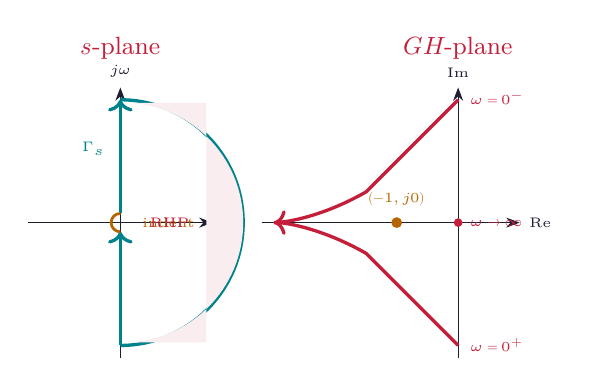
\begin{tikzpicture}[scale=0.78]
  % s-plane
  \begin{scope}[xshift=0cm]
    \draw[axis] (-1.5,0) -- (1.5,0) node[right,font=\tiny] {$\sigma$};
    \draw[axis] (0,-2.2) -- (0,2.2) node[above,font=\tiny] {$j\omega$};
    \node[above,font=\small,color=myred] at (0,2.5) {$s$-plane};
    % Nyquist contour
    \draw[color=myteal, line width=1.2pt, ->] (0,0.15) -- (0,2.0);
    \draw[color=myteal, line width=1.2pt] (0,2.0) arc(90:-90:2.0);
    \draw[color=myteal, line width=1.2pt, ->] (0,-2.0) -- (0,-0.15);
    % Indentation at origin
    \draw[color=myamber, line width=1.0pt] (0,0.15) arc(90:270:0.15);
    \node[left,font=\tiny,color=myteal] at (-0.1,1.2) {$\Gamma_s$};
    \node[right,font=\tiny,color=myamber] at (0.2,0) {indent};
    % RHP shading hint
    \fill[myred!8] (0.05,-1.95) arc(-90:90:1.95) -- (0.05,1.95) -- (1.4,1.95) -- (1.4,-1.95) -- cycle;
    \node[font=\tiny,color=myred] at (0.8,0) {RHP};
  \end{scope}
  % GH-plane
  \begin{scope}[xshift=5.5cm]
    \draw[axis] (-3.2,0) -- (1.0,0) node[right,font=\tiny] {Re};
    \draw[axis] (0,-2.2) -- (0,2.2) node[above,font=\tiny] {Im};
    \node[above,font=\small,color=myred] at (0,2.5) {$GH$-plane};
    % Nyquist plot (Type 1, 2nd order)
    \draw[color=myred, line width=1.2pt, ->]
      (0,-2.0) .. controls (-0.4,-1.6) and (-1.0,-1.0) .. (-1.5,-0.5)
      .. controls (-2.2,-0.1) and (-2.8,0) .. (-3.0,0);
    \draw[color=myred, line width=1.2pt]
      (0,2.0) .. controls (-0.4,1.6) and (-1.0,1.0) .. (-1.5,0.5)
      .. controls (-2.2,0.1) and (-2.8,0) .. (-3.0,0);
    % Large semicircle maps to origin
    \fill[myred] (0,0) circle (2pt);
    \node[right,font=\tiny,color=myred] at (0.05,0) {$\omega\to\infty$};
    % -1,0 point
    \fill[myamber] (-1,0) circle (2.5pt);
    \node[above,font=\tiny,color=myamber] at (-1,0.12) {$(-1,j0)$};
    % Labels
    \node[right,font=\tiny,color=myred] at (0.05,-2.0) {$\omega=0^+$};
    \node[right,font=\tiny,color=myred] at (0.05,2.0) {$\omega=0^-$};
  \end{scope}
\end{tikzpicture}
\end{tcolorbox}

%═══════════════════════════════════════════════════════════════════════════════
\section{Nyquist Stability Criterion}
%═══════════════════════════════════════════════════════════════════════════════

\begin{tcolorbox}[masonbox]
\textbf{Nyquist Stability Criterion:} Based on the \textbf{Principle of the Argument} (Cauchy's theorem). For a closed-loop system with open-loop transfer function $G(s)H(s)$:
$$N = Z - P$$
where:
\begin{itemize}[leftmargin=*, itemsep=2pt, topsep=2pt]
  \item $N$ = number of \textbf{clockwise encirclements} of the $(-1, j0)$ point by the Nyquist plot of $G(j\omega)H(j\omega)$.
  \item $Z$ = number of \textbf{closed-loop poles} in the RHP (zeros of $1+GH$).
  \item $P$ = number of \textbf{open-loop poles} of $G(s)H(s)$ in the RHP.
\end{itemize}
\textbf{For stability:} $Z = 0$, therefore $N = -P$ (i.e., $P$ \textit{counter-clockwise} encirclements if $P \neq 0$; no encirclements if $P = 0$).
\end{tcolorbox}

\subsection{Applying the Nyquist Criterion --- Step by Step}

\begin{enumerate}[label=\textbf{Step \arabic*:}, leftmargin=2.5cm, itemsep=4pt]
  \item Determine $P$ = number of open-loop poles of $G(s)H(s)$ in the RHP.
  \item Sketch the Nyquist plot of $G(j\omega)H(j\omega)$ for $\omega: 0^+ \to +\infty$.
  \item Mirror the plot about the real axis for $\omega: -\infty \to 0^-$.
  \item Handle poles on the $j\omega$-axis by indenting the contour (small semicircle of radius $\varepsilon\to0$).
  \item Count $N$ = net clockwise encirclements of $(-1, j0)$.
  \item Compute $Z = N + P$. If $Z = 0$: \textbf{stable}. If $Z > 0$: \textbf{unstable} ($Z$ RHP poles).
\end{enumerate}

\begin{tcolorbox}[examplebox, title={Example: $G(s)H(s) = K/[s(s+1)(s+2)]$, find stability range}]
\textbf{Open-loop poles:} $s=0$ (on $j\omega$-axis), $s=-1$, $s=-2$ (all in LHP). So $P=0$.

\textbf{Nyquist plot} crosses the negative real axis at $\omega_{pc}$ where $\angle G(j\omega)H(j\omega) = -180°$.

At $\omega_{pc}$: $\angle = -90° - \tan^{-1}(\omega) - \tan^{-1}(\omega/2) = -180°$
$\Rightarrow \tan^{-1}(\omega) + \tan^{-1}(\omega/2) = 90°$
$\Rightarrow \omega_{pc} = \sqrt{2}$ rad/s.

$|G(j\sqrt{2})H(j\sqrt{2})| = \dfrac{K}{\sqrt{2}\cdot\sqrt{3}\cdot\sqrt{4}} = \dfrac{K}{2\sqrt{6}}$

\textbf{For stability:} $N=0$ requires the plot does not encircle $(-1,j0)$:
$$\frac{K}{2\sqrt{6}} < 1 \;\Rightarrow\; K < 2\sqrt{6} \approx 4.9$$
\textbf{Gain Margin:} $GM = 2\sqrt{6}/K$. For $K=1$: $GM = 2\sqrt{6} \approx 4.9$ (13.8 dB).
\end{tcolorbox}

\subsection{Simplified Nyquist Criterion (Minimum Phase Systems)}

\begin{tcolorbox}[formulabox, title={For Minimum Phase Systems ($P=0$)}]
A minimum phase system (no open-loop RHP poles or zeros) is \textbf{closed-loop stable} if and only if the Nyquist plot of $G(j\omega)H(j\omega)$ does \textbf{not encircle} the $(-1, j0)$ point.\\[4pt]
Equivalently (from Bode plot): \textbf{stable} if $|G(j\omega_{pc})H(j\omega_{pc})| < 1$, i.e., $GM > 0$ dB \textbf{AND} $PM > 0°$.
\end{tcolorbox}

\begin{tcolorbox}[exambox, title={Exam Tips --- Nyquist Criterion}]
\begin{itemize}[leftmargin=*, itemsep=3pt, topsep=0pt]
  \item \textbf{$N = Z - P$} --- memorise this. $Z=0$ for stability.
  \item For \textbf{minimum phase} systems ($P=0$): stable iff no encirclement of $(-1,j0)$.
  \item \textbf{Clockwise} encirclement = positive $N$; \textbf{counter-clockwise} = negative $N$.
  \item Poles on $j\omega$-axis (e.g., integrators): indent contour to the right; the large semicircle maps to origin.
  \item The Nyquist plot is the \textbf{mirror image} of the polar plot about the real axis.
  \item \textbf{$(-1,j0)$ point} is the critical point --- corresponds to $|GH|=1$ and $\angle GH = -180°$.
\end{itemize}
\end{tcolorbox}

%═══════════════════════════════════════════════════════════════════════════════
\section{Performance Specifications in Frequency Domain}
%═══════════════════════════════════════════════════════════════════════════════

\begin{tcolorbox}[defbox]
\textbf{Frequency Domain Specifications} describe the closed-loop system's behaviour in terms of its frequency response $T(j\omega) = C(j\omega)/R(j\omega)$. They are directly related to time-domain performance.
\end{tcolorbox}

\subsection{Closed-Loop Frequency Response Specifications}

\begin{tabularx}{\linewidth}{|B{3.2cm}|>{\centering\arraybackslash}p{2.0cm}|X|}
\hline
\rowcolor{hdrteal}
\multicolumn{1}{|>{\centering\arraybackslash}p{3.2cm}|}{\textbf{\color{myteal}Specification}} &
\multicolumn{1}{>{\centering\arraybackslash}p{2.0cm}|}{\textbf{\color{myteal}Symbol}} &
\multicolumn{1}{>{\centering\arraybackslash}X|}{\textbf{\color{myteal}Definition}} \\
\hline
Resonant Peak & $M_r$ & Maximum value of $|T(j\omega)|$. Indicates relative stability; high $M_r$ means low damping. \\
\hline
\rowcolor{rowalt}
Resonant Frequency & $\omega_r$ & Frequency at which $|T(j\omega)|$ is maximum. \\
\hline
Bandwidth & $\omega_{BW}$ & Frequency at which $|T(j\omega)|$ drops to $1/\sqrt{2}$ ($-3$ dB) of its DC value. Indicates speed of response. \\
\hline
\rowcolor{rowalt}
Cutoff Rate & --- & Rate at which $|T(j\omega)|$ decreases beyond $\omega_{BW}$; indicates noise rejection. \\
\hline
\end{tabularx}

\subsection{Formulas for Second-Order System}

\begin{tcolorbox}[formulabox, title={Closed-Loop Frequency Response --- 2nd Order}]
For $T(s) = \omega_n^2/(s^2+2\zeta\omega_n s+\omega_n^2)$:
$$|T(j\omega)| = \frac{1}{\sqrt{(1-u^2)^2 + (2\zeta u)^2}}, \quad u = \omega/\omega_n$$
\textbf{Resonant frequency:} $\omega_r = \omega_n\sqrt{1-2\zeta^2}$ \quad (exists only for $\zeta < 1/\sqrt{2} \approx 0.707$)\\[4pt]
\textbf{Resonant peak:} $M_r = \dfrac{1}{2\zeta\sqrt{1-\zeta^2}}$ \quad (for $\zeta < 0.707$)\\[4pt]
\textbf{Bandwidth:} $\omega_{BW} = \omega_n\sqrt{(1-2\zeta^2)+\sqrt{4\zeta^4-4\zeta^2+2}}$
\end{tcolorbox}

\subsection{Relation Between Frequency and Time Domain Specs}

\begin{tabularx}{\linewidth}{|B{3.4cm}|>{\centering\arraybackslash}X|>{\centering\arraybackslash}X|}
\hline
\rowcolor{hdrgray}
\multicolumn{1}{|>{\centering\arraybackslash}p{3.4cm}|}{\textbf{Freq. Domain}} &
\textbf{\color{myamber}Relation} & \textbf{\color{mygreen}Time Domain Equivalent} \\
\hline
High $\omega_{BW}$ & $\omega_{BW} \propto \omega_n$ & Faster rise time, faster response \\
\hline
\rowcolor{rowalt}
High $M_r$ & $M_r \uparrow$ as $\zeta \downarrow$ & High overshoot $M_p$ \\
\hline
$M_r = 1$ & $\zeta \geq 0.707$ & No overshoot (overdamped/critically) \\
\hline
\rowcolor{rowalt}
Phase Margin & $PM \approx 100\zeta$ (for $\zeta < 0.7$) & Damping ratio $\zeta$ \\
\hline
Gain Margin & Larger GM & More stable, less sensitive to gain \\
\hline
\rowcolor{rowalt}
$\omega_{gc}$ & $\omega_{gc} \approx \omega_{BW}$ & Bandwidth approximation \\
\hline
\end{tabularx}

\begin{tcolorbox}[tikzbox, title={Closed-Loop Frequency Response (Resonance Peak)}]
\centering
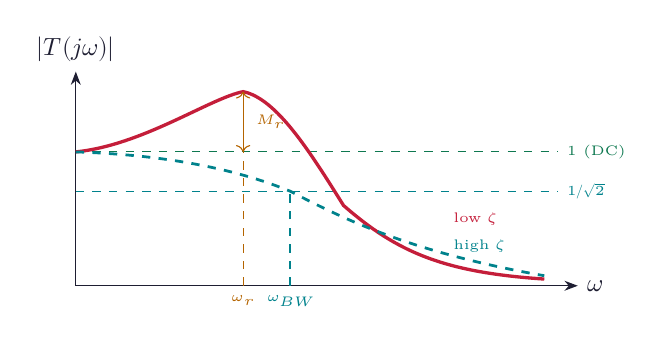
\begin{tikzpicture}[scale=0.85]
  \draw[axis] (0,0) -- (7.5,0) node[right,font=\small] {$\omega$};
  \draw[axis] (0,0) -- (0,3.2) node[above,font=\small] {$|T(j\omega)|$};
  % DC value = 1
  \draw[dashed,color=mygreen,thin] (0,2) -- (7.2,2) node[right,font=\tiny,color=mygreen] {$1$ (DC)};
  % -3dB line
  \draw[dashed,color=myteal,thin] (0,1.414) -- (7.2,1.414) node[right,font=\tiny,color=myteal] {$1/\sqrt{2}$};
  % Low damping curve (zeta=0.3)
  \draw[color=myred,line width=1.2pt]
    (0,2) .. controls (1,2.1) and (2,2.8) .. (2.5,2.9)
    .. controls (3,2.8) and (3.5,2.0) .. (4,1.2)
    .. controls (4.8,0.5) and (5.5,0.2) .. (7,0.1);
  % High damping curve (zeta=0.7)
  \draw[color=myteal,line width=1.0pt,dashed]
    (0,2) .. controls (1.5,1.95) and (2.5,1.7) .. (3.2,1.414)
    .. controls (4,1.0) and (5,0.5) .. (7,0.15);
  % Mr annotation
  \draw[<->,color=myamber,thin] (2.5,2) -- (2.5,2.9);
  \node[right,font=\tiny,color=myamber] at (2.55,2.45) {$M_r$};
  \draw[dashed,color=myamber,thin] (2.5,0) node[below,font=\tiny,color=myamber] {$\omega_r$} -- (2.5,2.9);
  % BW annotation
  \draw[dashed,color=myteal,thin] (3.2,0) node[below,font=\tiny,color=myteal] {$\omega_{BW}$} -- (3.2,1.414);
  % Legend
  \node[right,font=\tiny,color=myred] at (5.5,1.0) {low $\zeta$};
  \node[right,font=\tiny,color=myteal] at (5.5,0.6) {high $\zeta$};
\end{tikzpicture}
\end{tcolorbox}

\begin{tcolorbox}[exambox, title={Exam Tips --- Frequency Domain Specs}]
\begin{itemize}[leftmargin=*, itemsep=3pt, topsep=0pt]
  \item \textbf{$M_r > 1.3$} (about 2.3 dB) indicates poor relative stability (excessive overshoot).
  \item \textbf{$\omega_r < \omega_n$} always (resonant frequency is less than natural frequency).
  \item \textbf{$\omega_{BW} > \omega_n$} always (bandwidth exceeds natural frequency).
  \item \textbf{$PM \approx 100\zeta$} for $\zeta < 0.7$ --- very useful approximation in design.
  \item \textbf{Bandwidth} determines speed: wider BW = faster response but more noise.
  \item For $\zeta \geq 0.707$: $M_r = 1$ (no resonance peak); response is monotonically decreasing.
\end{itemize}
\end{tcolorbox}

%═══════════════════════════════════════════════════════════════════════════════
% QUICK REVISION --- MODULE 4
%═══════════════════════════════════════════════════════════════════════════════
\newpage
\begin{center}
  {\large\bfseries\color{myred} Quick Revision --- Module 4}\\[3pt]
  {\small\color{mydark} Frequency Response Analysis $|$ EC601}
\end{center}
\noindent{\color{myred}\rule{\linewidth}{1.2pt}}
\vspace{4pt}

\begin{tcolorbox}[formulabox, title={\textbf{Key Formulas at a Glance}}]
\begin{tabularx}{\linewidth}{B{5.2cm} X}
Frequency response          & $G(j\omega) = G(s)|_{s=j\omega}$ \\[2pt]
Gain Margin                 & $GM = 1/|G(j\omega_{pc})H(j\omega_{pc})|$ \\[2pt]
GM in dB                    & $GM_{dB} = -20\log|G(j\omega_{pc})|$ \\[2pt]
Phase Margin                & $PM = 180° + \angle G(j\omega_{gc})H(j\omega_{gc})$ \\[2pt]
Phase crossover freq        & $\omega_{pc}$: where $\angle GH = -180°$ \\[2pt]
Gain crossover freq         & $\omega_{gc}$: where $|GH| = 1$ (0 dB) \\[2pt]
Nyquist criterion           & $N = Z - P$; stable if $Z=0$ \\[2pt]
Resonant peak (2nd order)   & $M_r = 1/(2\zeta\sqrt{1-\zeta^2})$, $\zeta < 0.707$ \\[2pt]
Resonant frequency          & $\omega_r = \omega_n\sqrt{1-2\zeta^2}$ \\[2pt]
Bandwidth (2nd order)       & $\omega_{BW} = \omega_n\sqrt{(1-2\zeta^2)+\sqrt{4\zeta^4-4\zeta^2+2}}$ \\[2pt]
PM--damping relation        & $PM \approx 100\zeta$ (for $\zeta < 0.7$) \\[2pt]
Bode: simple pole slope     & $-20$ dB/dec above corner freq $\omega_c = 1/T$ \\[2pt]
Bode: double pole slope     & $-40$ dB/dec above $\omega_n$ \\[2pt]
Bode: phase at corner       & $-45°$ at $\omega_c$ for simple pole
\end{tabularx}
\end{tcolorbox}

\vspace{5pt}

\begin{tcolorbox}[defbox, title={\textbf{One-Line Definitions}}]
\begin{itemize}[leftmargin=*, itemsep=3pt, topsep=0pt]
  \item \textbf{Frequency Response:} System's steady-state response to sinusoidal input; $G(j\omega)$.
  \item \textbf{Polar Plot:} Locus of $G(j\omega)$ in complex plane as $\omega: 0\to\infty$.
  \item \textbf{Bode Plot:} Semi-log plots of magnitude (dB) and phase (deg) vs $\log\omega$.
  \item \textbf{Corner Frequency:} $\omega_c = 1/T$; slope changes by $\pm20$ dB/dec here.
  \item \textbf{Gain Crossover Freq $\omega_{gc}$:} Where $|GH|=1$ (0 dB); PM is measured here.
  \item \textbf{Phase Crossover Freq $\omega_{pc}$:} Where $\angle GH = -180°$; GM is measured here.
  \item \textbf{Gain Margin:} Factor by which gain can increase before instability; $GM > 0$ dB for stability.
  \item \textbf{Phase Margin:} Additional phase lag before instability; $PM > 0°$ for stability.
  \item \textbf{Nyquist Plot:} Polar plot of $GH(j\omega)$ for $\omega: -\infty\to+\infty$.
  \item \textbf{Nyquist Criterion:} $N=Z-P$; stable if $Z=0$ (no RHP closed-loop poles).
  \item \textbf{Resonant Peak $M_r$:} Maximum of $|T(j\omega)|$; indicates damping ($M_r\uparrow$ as $\zeta\downarrow$).
  \item \textbf{Bandwidth $\omega_{BW}$:} Freq where $|T|$ drops to $-3$ dB; indicates response speed.
  \item \textbf{Minimum Phase System:} No RHP poles or zeros; $P=0$; stable iff no encirclement of $(-1,j0)$.
\end{itemize}
\end{tcolorbox}

\vspace{5pt}

\begin{tcolorbox}[exambox, title={\textbf{Frequently Asked / Viva Questions}}]
\begin{enumerate}[leftmargin=*, topsep=0pt, label=\textbf{Q\arabic*.}, itemsep=8pt]
  \item \Q{What is the frequency response of a system?} The steady-state output-to-input ratio for sinusoidal inputs; obtained by substituting $s=j\omega$ in $G(s)$.
  \item \Q{What is the gain crossover frequency?} The frequency $\omega_{gc}$ where $|G(j\omega)H(j\omega)|=1$ (0 dB). Phase margin is measured here.
  \item \Q{What is the phase crossover frequency?} The frequency $\omega_{pc}$ where $\angle G(j\omega)H(j\omega)=-180°$. Gain margin is measured here.
  \item \Q{Define Gain Margin.} $GM = 1/|GH(j\omega_{pc})|$. It is the factor by which gain can be increased before instability. Stable if $GM > 1$ (0 dB).
  \item \Q{Define Phase Margin.} $PM = 180° + \angle GH(j\omega_{gc})$. Additional phase lag before instability. Stable if $PM > 0°$.
  \item \Q{State the Nyquist stability criterion.} $N = Z - P$. For stability $Z=0$, so $N=-P$. For minimum phase ($P=0$): no encirclement of $(-1,j0)$.
  \item \Q{What is $N$, $Z$, $P$ in Nyquist criterion?} $N$ = clockwise encirclements of $(-1,j0)$; $Z$ = RHP closed-loop poles; $P$ = RHP open-loop poles.
  \item \Q{What is the slope of Bode magnitude plot for a simple pole?} $-20$ dB/decade above the corner frequency $\omega_c = 1/T$.
  \item \Q{What is the resonant peak $M_r$?} Maximum value of closed-loop frequency response; $M_r = 1/(2\zeta\sqrt{1-\zeta^2})$ for 2nd order. Exists only for $\zeta < 0.707$.
  \item \Q{What is bandwidth?} Frequency at which $|T(j\omega)|$ drops to $1/\sqrt{2}$ ($-3$ dB) of DC value. Wider BW = faster response.
  \item \Q{Relation between PM and damping ratio?} $PM \approx 100\zeta$ for $\zeta < 0.7$. So $PM = 45°$ corresponds to $\zeta \approx 0.45$.
  \item \Q{What is a minimum phase system?} A system with no RHP poles or zeros and no time delay. Its Bode magnitude uniquely determines the phase.
\end{enumerate}
\end{tcolorbox}

\vspace{5pt}

\begin{tcolorbox}[tikzbox, title={\textbf{Stability Summary}}]
\begin{tabularx}{\linewidth}{|>{\centering\arraybackslash}X|>{\centering\arraybackslash}X|>{\centering\arraybackslash}X|}
\hline
\rowcolor{hdrteal}
\textbf{\color{myteal}Condition} & \textbf{\color{mygreen}Stable} & \textbf{\color{myred}Unstable} \\
\hline
Gain Margin & $GM > 1$ ($> 0$ dB) & $GM < 1$ ($< 0$ dB) \\
\hline
\rowcolor{rowalt}
Phase Margin & $PM > 0°$ & $PM < 0°$ \\
\hline
Nyquist ($P=0$) & No encirclement of $(-1,j0)$ & Encircles $(-1,j0)$ \\
\hline
\rowcolor{rowalt}
Nyquist (general) & $Z = N + P = 0$ & $Z = N + P > 0$ \\
\hline
Bode (min. phase) & $\omega_{gc} < \omega_{pc}$ & $\omega_{gc} > \omega_{pc}$ \\
\hline
\end{tabularx}
\end{tcolorbox}

\end{document}
